
\subsection{Countours and Bounding Boxes}

Contours formally identify a foreground object by identifying the coordinates of their perimeter. Figure \ref{fig:contour_polygon} shows the contour outlines of each foreground object from \ref{fig:bounding_boxes} which were located by using OpenCV's findContours function, which is based on the algorithm by Satoshi Suzuki \cite{satoshi_findContours}. Taking pixels at the extremities in the x and y direction for each contour is used to form bounding boxes as in Figure \ref{fig:bounding_boxes}. Bounding boxes can be used to determine the area, height, width and location of an object, which are important properties when trying to determine if an object is a vehicle, furthermore they store and compute more cheaply the irregular polyon of a contour. The bounding box dimensions and location are generated by the OpenCV function boundRect which takes a contour as a parameter and returns a bounding box's up-right rectangular contour, that is the top left corner coordinate and the box's width and height. 

\begin{figure}[H]
    \centering
    \centering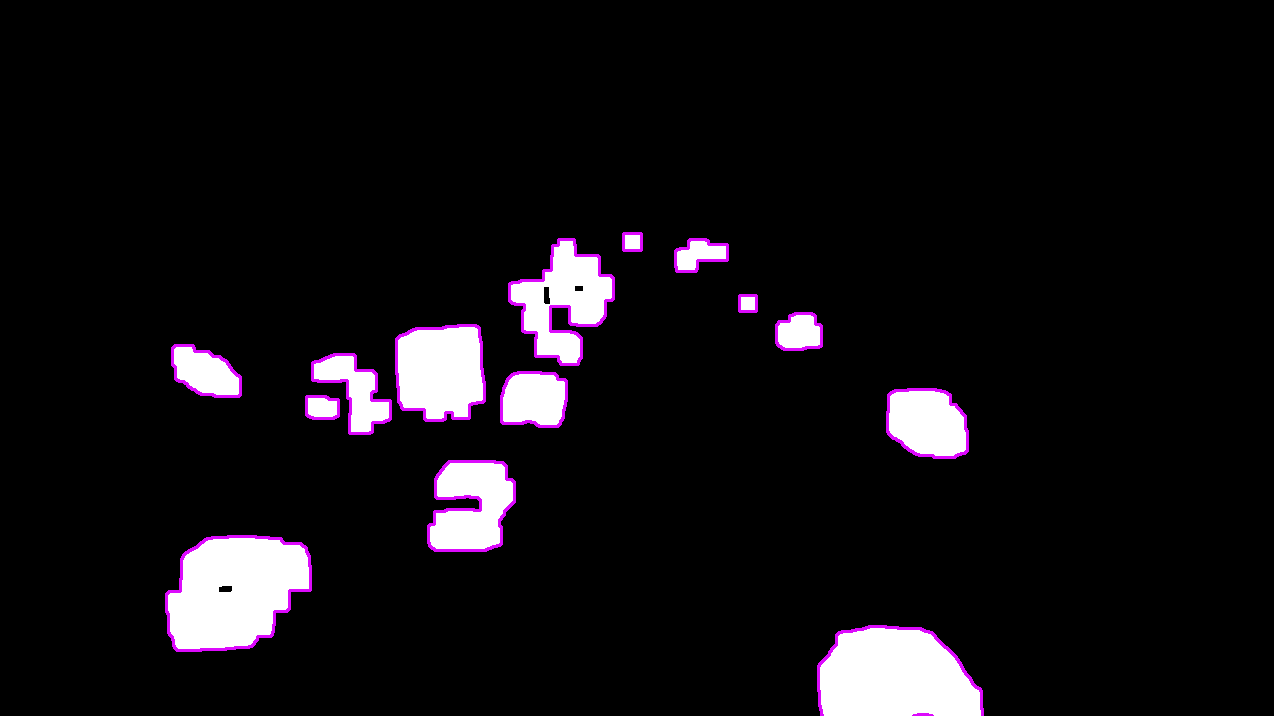
\includegraphics[width = 0.8\textwidth]{design/detection/bounding/mask_contours}
    \caption{Contours outlining foregroung mask objects.}
    \label{fig:contour_polygon}
\end{figure}
  
  
